\section{Introduction}\label{sec:introduction}

In the past few years, we have witnessed the rapid development of the blockchain industry; the influx of capital, users, and builders has made the entire blockchain industry reach unprecedented prosperity. However, since blockchain is still a brand new field and the infrastructure is not yet complete, there are also some problems behind the prosperity. The more prominent problem is the low TPS of the blockchain system, especially the largest public blockchain Ethereum \cite{website:Ethereum}, in the peak case \cite{website:Etherscan-chart}, can only process up to 23 transactions per second, which is far from the traditional centralized system. 

There are many reasons for the congestion of the Ethereum network, such as the POW \cite{website:POW} consensus algorithm (The Merge upgrade \cite{website:The-Merge} to POS \cite{website:POS} consensus now), the repeated execution of verification process of all transactions by nodes, and the serial execution of transactions; for the above reasons, many projects try to scale Ethereum to obtain higher throughput from different dimensions. Approach 1: New public blockchain, which is independent of Ethereum, using faster consensus algorithm or faster transaction execution to get higher TPs, such as BSC \cite{website:BSC}, Solana \cite{website:Solana}, Aptos \cite{website:Aptos}, etc; Approach 2: Ethereum Sidechain, using faster consensus algorithm and then regularly synchronizing to Ethereum, such as Polygon \cite{website:Polygon}, Optimism \cite{website:Optimism}, Arbitrum \cite{website:Arbitrum}, etc; Approach 3: ZK(E)VM, the Layer2 network of Ethereum, using ZK technology to solve the problem of repeated execution of transactions, such as Polygon Hermez \cite{website:Polygon-Hermez}, Zksync \cite{website:Zksync} and so on.

Obviously, in the long term, scaling is not the only problem that has to be solved in Ethereum even the whole blockchain. As there are many excellent teams working hard for scaling, we believe that the next important feature that should be implemented is privacy. Since the blockchain is a public ledger, all transactions that take place on chain are open and transparent, and the asset information of any address is also open and transparent. Excessive information transparency leads to (1) MEV problems, miners selectively package transactions according to the fee, resulting in transactions that are given low fees can not be processes, increasing the fee is the only way; (2) Huge asset address security problems, in the past year, the total assets stolen by hacher are about 2 billion; (3) User data ownership problems, both the assets information and transactions information of address are free to be monitored and used, which is contrary to the vision of Web3 \cite{website:Web3}. Therefore, when the scaling problem is solved, privacy will become the next urgent feature to be achieved.in the world of blockchain, privacy is not a new topic, it has long been studied and supported by the Zcash team \cite{website:Zcash}.

\subsection{Non Programmable Privacy}

In addition to the Zcash team, other public blockchains that implement private transactions include Monero \cite{website:Monero}, Dash \cite{website:Dash}, Grin \cite{website:Grin}, and others. However, these public chains lack programmability and can only be used for simple private transfer of assets. Consequently, their ecosystem development lags far behind Ethereum, which has become the largest public chain in the ecosystem due to its programmability, but Ethereum lacks privacy features.

Therefore, some projects have begun to explore ways to introduce privacy to Ethereum, such as the ZK-ZKRollup application zk.money \cite{website:zk.money} developed by the Aztec \cite{website:Aztec} team. However, the current zk.money product has been discontinued, mainly because it's privacy features only apply to simple single transfer scenarios. Given the current explosion of Defi applications, asset transfer is only one of the simplest financial scenarios, and therefore the user base is limited, while the maintenance costs continue to accrue.
\begin{figure}[!ht]
    \centering
    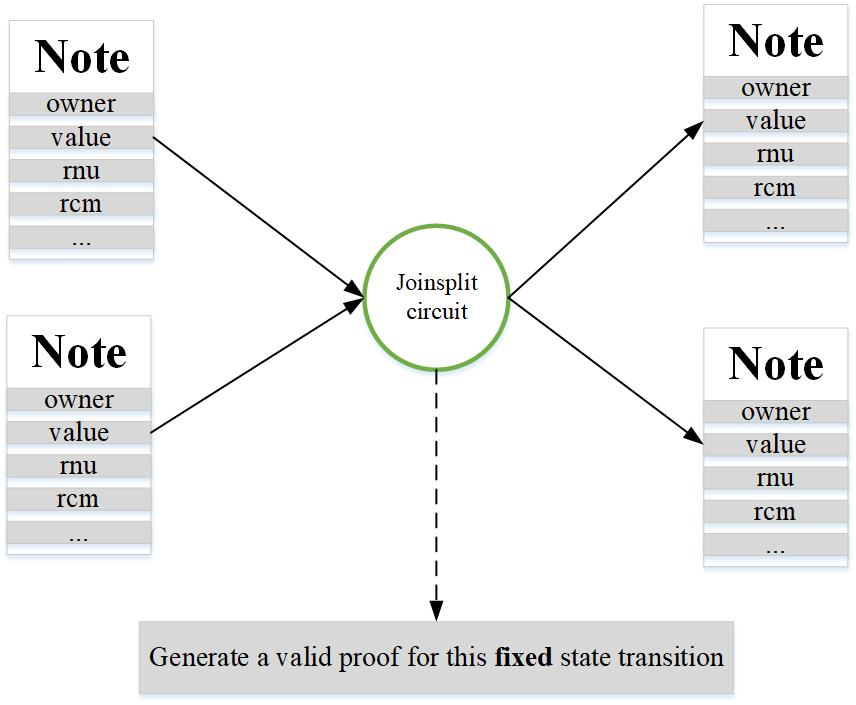
\includegraphics[width=0.4\textwidth]{Example of Non Programmable privacy.jpg}
    \caption{Example of Non Programmable Privacy}
    \label{fig:Example of Non Programmable Privacy}
\end{figure}

\figref{fig:Example of Non Programmable privacy} shows the simple logic of non programmable privacy. The value change logic corresponding to the input and output notes in Section \ref{section: sending-notes} are also fixed, generally in the form of ``A + B = C + D''. Manta Network \cite{website:Manta-network} is a public blockchain that supports user-defined token privacy transfers, and the privacy transaction 
constraint circuits of all fungible tokens can be used to reuse the above logic.

A ZK-ZKRollup application of a single scenario use case, is similar to a ZKRollup application of a single scenario use case. If you want to use the asset in other applications or for other use cases, you must cross the asset to another application through a bridge, which brings with it very poor user experience. Therefore, just as ZKRollups need to 
transition to ZK(E)VMs, ZK-ZKRollup also need to transition to ZK-ZKVMs (Appendix \ref{section: solidity-compatibility} explains how to get solidity compatibility).

\subsection{Programmable Privacy}

ZK-ZKVM has two main features (1) It's a privacy-first platform, not privacy-only. This means that users can choose the transaction type, public or private, depending on their need. Just similar to the Zcash;
(2) Programmability, you can deploy any smart contract, public or private, depending on the needs of the project side. Compared with non programmable privacy, the main difference is the logic of state transition in a note \ref{section: sending-notes}, \figref{fig:Difference between Non Programmable Privacy and Programmable Privacy} simply shows the difference 

\begin{figure}[!ht]
    \centering
    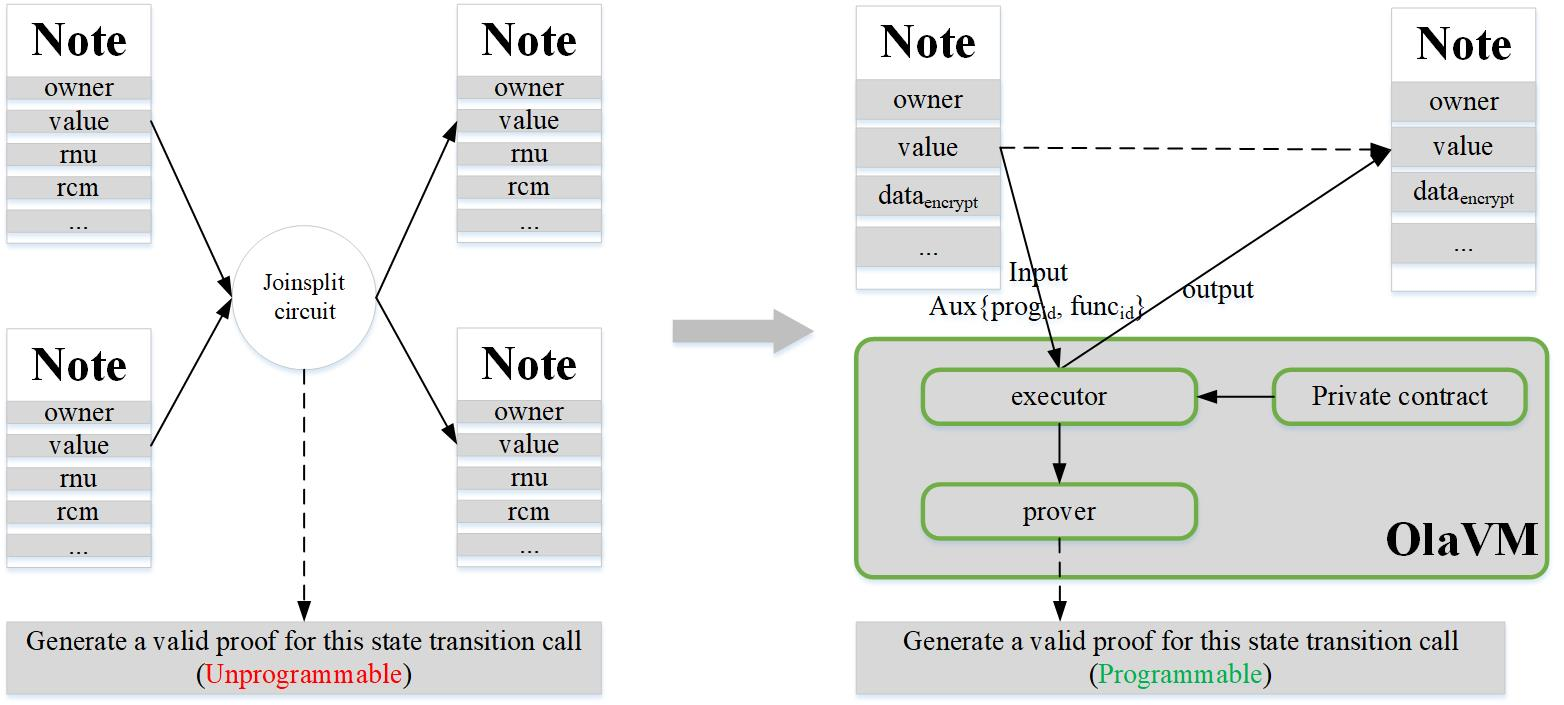
\includegraphics[width=0.6\textwidth]{Difference between Non Programmable Privacy and Programmable Privacy.jpg}
    \caption{Difference between Non Programmable Privacy and Programmable Privacy}
    \label{fig:Difference between Non Programmable Privacy and Programmable Privacy}
\end{figure}

The current projects focusing on programmable privacy are Aleo \cite{website:Aleo} and Aztec. Aleo is a 
privacy-first public blockchain, from Bitcoin \cite{website:BTC} to Ethereum to Zcash \cite{website:Zcash} to Aleo. It brings the public blockchain into a new era,
supporting programmable privacy. 
It has reached the testnet stage and supports developers to deploy privacy contracts on it; 
Aztec focuses on doing Layer2 programmable privacy for Ethereum, a project 
called Aztec3 \cite{website:Aztec3}, is still in development.

Before we clarify the different approaches to get programmability, we should give some explanations on Domain Specific Language (DSL) and General Purpose Language (GPL) \cite{website:DSL}.
DSL is defined as a computer programming language of limited expressiveness focused on a particular domain, limited expressiveness means it just supports a bare minimum of features 
needed to support its domain. You can't build an entire software system in a DSL; rather, you use a DSL for one particular aspect of a system. While GPL is defined as a general-purpose programming language

So there are often two ways to achieve programmability, one is to design a DSL, such as Circom \cite{website:Circom}, Pil \cite{website:Pil}, Noir \cite{website:Noir}, etc; the other is SCL, 
such as Cairo1.0 \cite{website:Cairo1.0}, Solidity \cite{website:Solidity}, Ola lang \cite{website:Ola-lang} and so on. As we have mentioned before, the main difference is that SCL supports more complex structures and has 
higher abstraction, it's more suitable for writing complex business logic and meanwhile, and DSL is more suitable for some simple computational expressions. 
Take Pil \cite{website:Pil} language as an example, you can directly use it to define a simple micro-op, such as ``A * B + C'', or ``A * B * C + D'' and other simple combinations. 
\tabref{table:Difference between DSL and SCL} briefly shows some of the differences between DSL and SCL.

\begin{table}[!ht]
    \centering
    \begin{tabular}{|c|c|c|c|c|c|}
        \hline
        \emph{Type} & \emph{Abstraction} & \emph{Process} & \emph{Difficulty} & \emph{Examples} & \emph{Notes} \\ 
        \hline
        DSL & low & program -> arith-ops -> ops gadgets & normal & \makecell{circom \\ noir \\ cairo} & \makecell{1. semantic analysis \\ 2. codeGen optimization} \\
        \hline
        \makecell{SCL \\ (ISA/VM)} & high & program -> bytecodes -> cpu circuit & hard & \makecell{solidity \\ cairo1.0 \\ ola lang} & \makecell{1. need a compiler \\2. re-use LLVM framework} \\
        \hline
    \end{tabular}
    \caption{Difference between DSL and SCL}
    \label{table:Difference between DSL and SCL}
\end{table}

If you want to prove a program written by DSL is executed correctly (this is what ZKDSL means), you may need to predefine some common operators, each of them corresponding to a circuit, called a gadget \cite{website:Gadget}. 
Developers can use these operators to implement desired functions, but it's difficult to handle the call and return logic between functions. Meanwhile, If you want to prove a program written by SCL is executed correctly (this is what ZKVM means), 
 you need to design corresponding constraints for each instruction, collectively referred to as CPU circuit; therefore, Any program will be compiled into 
 bytecodes composed of these instructions, and then constrained by the CPU circuit.

Ola achieved a customized SCL to get programmability even though it's harder to implement than DSL, because we could get benefits from it as follows:
 \begin{itemize}
 \item A higher abstraction and programmable language, allowing developers to write smart contracts with arbitrary logic;
 \item A full-featured zk-friendly VM can be designed to achieve higher system performance;
 \item LLVM-based compiler can be more easily compatible with other advanced programming languages.
\end{itemize}

\subsection{Full-featured ZK-friendly ZKVM}

As mentioned earlier, the best way to achieve programmability is to design a ZKVM with a custom Instruction Set Architecture, a custom smart contract language, and a custom compilation, etc. 
ZKVM is a virtual machine that can execute any program and at the same time generate a zero-knowledge proof of the correctness of the execution process. Therefore, the speed of proof generation 
is very critical, and it will directly affect the performance of the entire system.

The key to obtaining a full-featured zk-friendly ZKVM is how to obtain(1)the smallest execution trajectory; (2)the most concise state transition constraint logic; (3)the fastest 
zero-knowledge proof algorithm. The smallest execution trajectory means: for the same computational logic, OlaVM \cite{website:OlaVM} can be expressed with the least instructions, the main technical means are the 
support for non-deterministic computation at the computational level, and the register-based design is used at the memory access level; The most concise state transition constraint logic means: 
for the same computational logic, OlaVM \cite{website:OlaVM} can constrain the entire execution trajectory with the least polynomials and the smallest order. The main means is to obtain the instruction with the least 
number of instructions through the Algebraic RISC architecture. The number of Instruction Set Architecture determines the complexity of Cpu constraints; faster zero-knowledge proof algorithm 
Meaning: For the same calculation, OlaVM \cite{website:OlaVM} can complete the proof generation process in less time, which mainly depends on the Godilocks \cite{website:Goldilocks} field, a finite field less than 64bit, compared to the 
SNARK system based on large bit width elements of elliptic curves, based on The STARK algorithm of the Goldilocks \cite{website:Goldilocks} field can be executed faster.

Subsequent chapters will explain in detail Ola's design philosophy and design specifications for obtaining a Full-featured ZK-friendly ZKVM. As the first programmable privacy layer network 
based on ZKVM, Ola will support the following scenarios for different subjects:

\begin{itemize}
\item For Developers
    \begin{itemize}
    \item Developers can freely choose to deploy public contracts(Account-based), privacy contracts(Note-based), and ordinary contracts(Account and Note-based)
        \begin{enumerate}
        \item For public contracts, Ola functions as a ZKVM;
        \item For privacy contracts, Ola functions as a ZK-ZKVM;
        \item For ordinary contracts, Ola functions as a ZK-ZKVM or ZKVM, depending on the user's transaction type;
        \end{enumerate}
    \item Transfer of assets between public and private accounts
    \item Intra-contract, no bridge contract is required, supported by default;
    \item Cross-contract, a bridge contract is required;
    \end{itemize}
\item For Users
    \begin{itemize}
    \item For ordinary contract types, users can freely choose the transaction type;
    \item For public/private contract types, users can only execute transactions of the corresponding type;
    \item Users have a view key to disclose executed private transactions;
    \item Ola supports the update of the view key so that after the view key is exposed, the privacy transactions executed by the user in the future will always be parsed;
    \item Ola supports asset transfers between public and private accounts;
    \end{itemize}
\end{itemize}
\subsection{Outline}

Ola is a full stack developer framework for zero-knowledge applications, the whole framework is shown as \figref{fig:Ola framework}:
\begin{figure}[!ht]
    \centering
    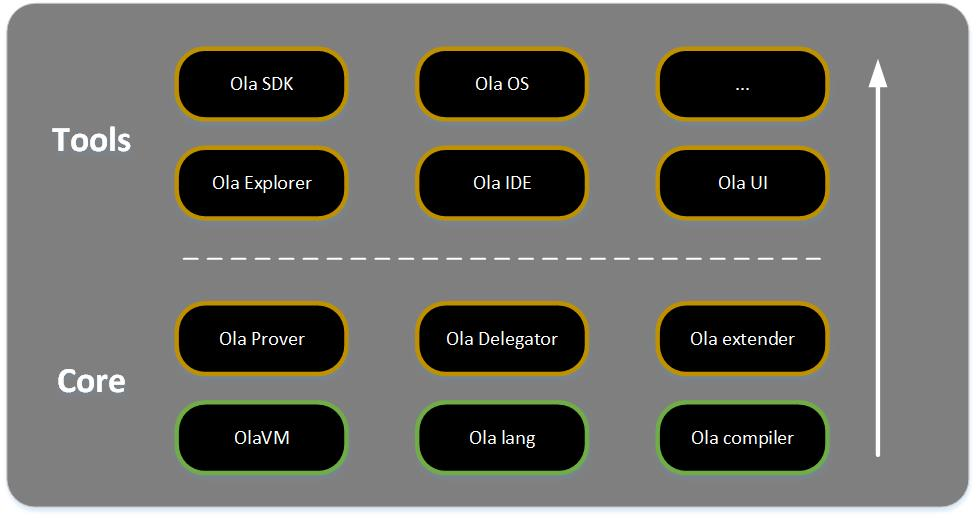
\includegraphics[width=0.6\textwidth]{vm/Ola framework.jpg}
    \caption{Ola framework}
    \label{fig:Ola framework}
\end{figure}

The green borders refers to the modules we have completed implementation, and others stand for the modules we will implement in the future. In the remaining sections of this whitepaper, we will introduce those modules 
as follows:
\begin{itemize}
    \item Section \ref{sec:olavm-a-full-featured-zk-friendly-zkvm} mainly describes the design of Ola's virtual machine, including our zk-friendly design schemes;
    \item Section \ref{sec:ola-lang} mainly describes the design of the customized smart contract language, Ola-lang and the framework of Ola compiler based LLVM;
    \item Section \ref{sec:ola-compiler} mainly describes the design of Ola compiler;
    \item Section \ref{sec:zk-zkvm} mainly describes key points on achieving privacy;
    \item Section \ref{sec:algorithms} mainly describes algorithms used in Ola, including zk and hardware acceleration algorithms;
    \item Section \ref{section:appendix} mainly describes the key features we researched to be supported in the future and our frameworks around that;
    \item Section \ref{sec:glossary} mainly describes some basic notations;
\end{itemize}

